\chapter{Principios físicos}

El objetivo de esta clase es familiarizarze con los conceptos de combinación de banda y firma espectral.



\section{Combinación de bandas}
Se realizarán combinaciones de bandas teniendo en cuenta la respuesta espectral de los distintos usos y coberturas.

%desarrollar un poco

\subsection{Combinación color real}\label{sec:colorreal}

Abra la imagen \begin{center} \directory{S2B\_MSIL2A\_2018-01-31.dim}.
\end{center} seleccione \menu{Open RGB image windows} haciendo click derecho sobre el nombre. La nueva ventana (Figura \ref{fig:RGB} Guía Clase 1), le permitirá elegir la combinación de bandas. Por defecto aparecerá la combinación color real que utiliza las bandas del \emph{rojo (B4)}, \emph{verde (B3)} y \emph{azul (B2)} de \emph{Sentinel-2}. Despliegue haciendo click en \menu{OK}.

La imagen se observa en colores similares a los que vería el ojo humano. Es así que la vegetación sana aparece en tonalidades de verde, la vegetación senescente o de escasa cobertura en tonos de marrón o amarillo y los suelos recientemente cosechados o compactados se observan brillantes. Esta combinación de bandas posibilita una buena diferenciación de los cuerpos de agua, resaltando características como la presencia de sedimentos o floraciones algales y la profundidad.

Utilice el mapa con puntos de interés (Figura \ref{fig:mapa} Guía Clase 1) para identificar y familiarizarse con los diferentes usos y coberturas. Explore la imagen utilizando las herramientas de navegación y zoom. Compare color, tono y textura.


\subsection{Combinación infrarrojo color}
\label{sec:infrarrojocolor}

Seleccione \menu{Open RGB image windows}, elija las bandas \emph{infrarrojo cercano (B8)}, \emph{verde(B4)} y \emph{azul(B3)} de \emph{Sentinel-2}. Despliegue haciendo click en \menu{OK}.

En esta combinación la vegetación leñosa como el bosque, varía en tonos rojizos y, la vegetación herbacea como los pastizales y cultivos, se visualizan en magenta. Los suelos se muestran en diversos tonos de verde y las áreas urbanas aparecen en cian tendiendo al azul cuando se encuentran densamente pobladas.
Esta combinación de bandas es útil para el estudio de la vegetación ya que resalta la relación entre la longitud de onda del rojo y del infrarrojo cercano.

Utilice el mapa con puntos de interés (Figura \ref{fig:mapa} Guía 1) e identifique diferentes tipos de vegetación. Explore la imagen utilizando las herramientas de navegación y zoom. Compare color, tono y textura.

\subsection{Combinación vegetación sana}
\label{sec:vegetacionsana}

Seleccione \menu{Open RGB image windows} haciendo click derecho sobre el nombre de la imagen. Elija las bandas \emph{infrarrojo cercano (B8)}, \emph{infrarrojo onda corta(B11)} y \emph{azul(B2)} de \emph{Sentinel-2}. Despliegue haciendo click en \menu{OK}.

La vegetación saludable aparece en tonos de rojos, marrones, naranjas y amarillos. Los suelos pueden observarse en variedades de verde y marrón. Los suelos sin cobertura vegetal estarán en azul intenso, mientras que aquellos con vegetación en crecimiento se mostrarán rosados. El agua clara y profunda se percibe oscura mientras que, si es poco profunda o contiene sedimentos, aparecerá con tonos de azul más claro.
La adición de la banda del infrarrojo de onda corta aumenta la sensibilidad para identificar estrés hídrico y variaciones del contenido de humedad en la vegetación y suelos.

Utilice el mapa con puntos de interés para identificar diferentes tipos de vegetación (Figura \ref{fig:mapa}, Guía Clase 1). Explore la imagen utilizando las herramientas de navegación y zoom. Compare color, tono y textura.

\section{Firmas espectrales}


En esta ocasión se analizará el comportamiento espectral de diferentes usos y coberturas.

\subsection{Puntos de muestreo}

El siguiente paso será seleccionar puntos de interés para evaluar el comportamiento espectral de los diferentes usos y coberturas del suelo. Se utilizará la herramienta \menu{pin placing tool} (Figura \ref{fig:pin}) para tomar puntos de muestreo, sobre los cuales luego se graficarán las firmas espectrales.

\begin{figure}[h!]
    \centering
    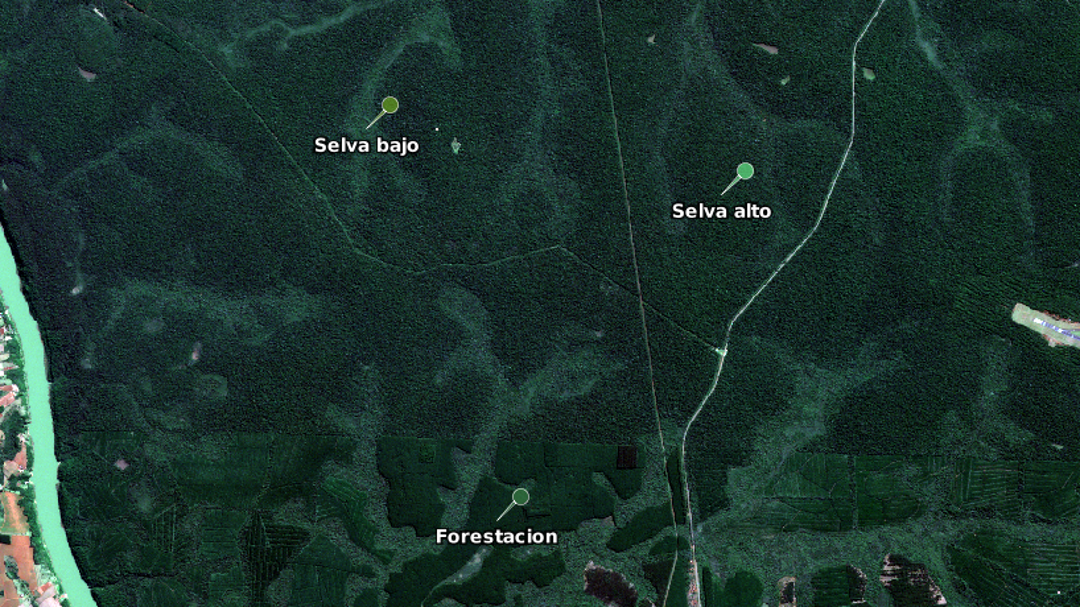
\includegraphics[width=0.05\textwidth]{fig:pin.png}
    \caption{Herramienta Pin placing tool.}
    \label{fig:pin}
\end{figure}

Visualice la imagen en combinación de bandas vegetación sana e identifique un parche homogéneo de selva paranense. Seleccione la herramienta \menu{pin placing tool} y haga click sobre la imagen para agregar un Pin (Figura \ref{fig:selva}).

\begin{figure}[h!]
    \centering
    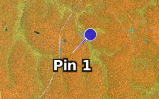
\includegraphics[width=0.2\textwidth]{fig:pin-selva.png}
    \caption{Pin en un parche homogéneo de selva paranaense.}
    \label{fig:selva}
\end{figure}

Para cambiar las características del Pin vaya a \menu{View>Tool Windows>Pin Manager} y aparecerá una nueva ventana con los datos del punto. Seleccione el nombre del Pin en la columna \menu{label} y cambielo por "selva paranaense". En la columna \menu{color} asigne el color deseado.

\subsection{Visualización de firmas espectrales}

Ahora visualice la firma espectral correspondiente al Pin creado. Seleccione \menu{Optical>Spectrum View} y se desplegará una nueva ventana. Haga click derecho sobre el gráfico y elija \menu{Auto Range>Both Axes}. Para obtener la firma espectral del Pin, seleccione la herramienta \menu{Show spectra for all pins} (Figura \ref{fig:spectral-signature}).


Realice y compare las firmas espectrlales de bosque implantado, cultivo, suelo sin cobertura vegetal y cuerpo de agua. Recuerde insertar un pin para cada cobertura y modifique sus caracteristicas con el nombre nombre correspondiente.

\begin{figure}[h!]
    \centering
    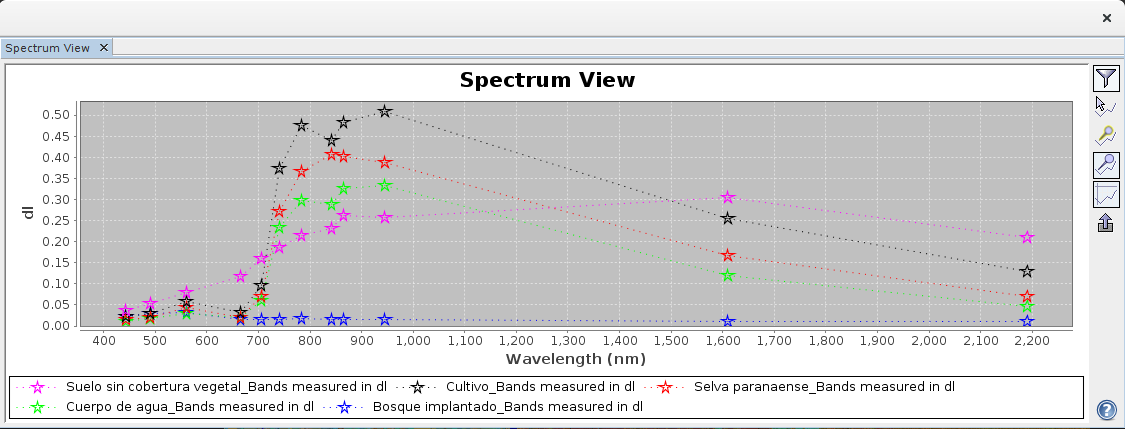
\includegraphics[width=0.7\textwidth]{fig:spectral-signature.png}
    \caption{Ejemplo de firmas espectrales.}
    \label{fig:spectral-signature}
\end{figure}

\section{Actividad práctica}
\begin{enumerate}
  \item Despliegue las tres combinaciones de la imagen utilizando múltiples visualizadores e identifique la intersección entre el río Paraná y el río Iguazú.
  \begin{enumerate}
  \item Compare el color y tono de ambos ríos. En base a la interpretación visual ¿Qué combinación de bandas considera la más adecuada para identificar la presencia de sedimentos? ¿Qué río tiene mayor concentración de sedimentos?.

  \item  Identifique la ciudad de Puerto Iguazú y analice el área urbana. ¿En qué combinación se puede ver con mayor nitidez la red víal?.

  \item  Identifique el embalse Urugua-í y compare la presencia de sedimentos con los ríos Paraná e Iguazú. ¿Cuál de ellos presenta menor concentración?.
\end{enumerate}

  \item Identifique la Selva Paranaense y el Bosque Implantado
  \begin{enumerate}
    \item  Compare el color y tono para la combinación de bandas color natural.
    \item  Compare el color y tono para la combinación de bandas infrarrojo color.
    \item  Compare el color y tono para la combinación "vegetación sana".
    \item  ¿En qué combinación encuentra mayor heterogeneidad? ¿Cuál considera que es la más útil para separar diferentes tipos de vegetación?
  \end{enumerate}

  \item Compare un cultivo con cobertura vegetal y un lote de suelo sin cobertura  ¿Qué combinación considera más útil para medir heterogeneidad de un suelo sin cobertura vegetal? ¿y para suelos con vegetación?


  \item Seleccione la imagen en combinación color real. Inserte un pin para el río Paraná, río Iguazú y embalse Urugua-í. Modifique sus caracteristicas y grafique sus firmas espectrales.
  \begin{enumerate}
      \item Compare las tres firmas espectrales. Analice el patrón de reflectancia. ¿Presentan todas el mismo patrón?
      \item Identifique picos y valles de reflectancia. ¿Qué cuerpo de agua presenta mayor reflectancia en el visible-NIR? ¿Cuál presenta menor? Analice los factores biofísicos que modelan este comportamiento.
    \end{enumerate}

  \item Seleccione la imagen en combinación vegetación sana. Inserte un pin para selva paranaense, bosque implantado, cultivo y suelo sin cobertura vegetal. Modifique sus características y grafique sus firmas espectrales.
  \begin{enumerate}
    \item Analice las cuatro firmas espectrales teniendo en cuenta los picos y valles de reflectancia de acuerdo a la longitud de onda. ¿En qué longitudes de onda presenta mayor reflectancia la vegetación? ¿En cuáles presenta menor reflectancia? Explique teniendo en cuenta los parámetros fisiológicos que modelan este comportamiento.
    \item Compare una firma de vegetación fotosintéticamente activa (e.g. selva paranaense), con otra de suelo sin cobertura vegetal. ¿Pueden diferenciarse en el visible? ¿Y en el infrarrojo cercano? Analice donde se observan mayores diferencias.
  \end{enumerate}
	\item Identifique un área urbana, grafique su firma espectral y compare con el resto de las coberturas. ¿Qué diferencias observa con el suelo sin cobertura vegetal?
  \end{enumerate}

Estas preguntas y actividades no serán evaluadas. Su objetivo es discutirlas en el foro de consultas e intercambio de la clase.

%Ver cómo manejar el tema de borrar pines en las comparaciones
% Añadir al anexo las longitudes de onda x mision satelital.
